% $Id$

\chapter{Non-kernel machine example}
\label{non_kernel_machine_tutorial}
\minitoc

In this example, we will use the same dataset used in Chapter 8 and a non-kernel machine to classify conditions `A' and `B'. As non-kernel machines build the model based on the original features and not based on the similarity between samples they can be computationally expensive if the number of features is very large. However, some algorithms only exist in primal form and could be of interest (for example LASSO, Tibshirani, 1996). In this tutorial, we will select a single channel (one on which there is signal) of the same ECoG data we used in the previous chapter and use the L1-SVM machine that selects a subset of informative features during model estimation.
\\

This tutorial will be quite short as most information is already introduced in chapter \ref{semisimulated_ecog} and in this tutorial we build on top of that. So the reader is strongly advised to do that tutorial first before proceeding to this one.

\section{GUI analysis}

%---------------------------------------------------------------------

\subsection{Data \& Design}

You will need to replicate, exactly, the procedure followed in the previous chapter. Follow step by step subsection \ref{sssec:data_and_design_semisim_gui} in order to finish inputting the data.

%---------------------------------------------------------------------

\subsection{Prepare feature set}

\begin{itemize}
    \item First replicate, exactly, the procedure followed in the previous chapter in order to build the first feature set, `All', used in that chapter. Follow step by step subsection \ref{sssec:feature_set_semisim_gui} in order to do this.
    
    \item Then build a second feature set (`Chan3'), that will include only channel 3 and time points the same as before, [-100 1100]ms around onset. The final configuration of this feature set should look like figure \ref{fig:non_kernel_gui_prepare_featureSet_3}

\end{itemize}

\begin{figure}[!h]
  \centering
		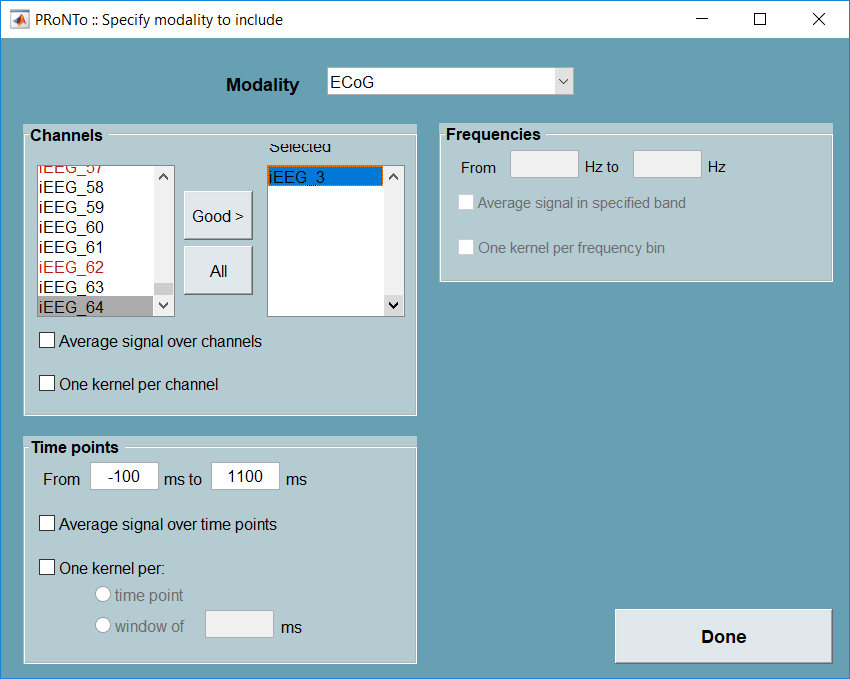
\includegraphics[scale=0.55]{images/Tutorial/v3/non_kernel_machine_tutorial/non_kernel_gui_prepare_featureSet_3.png}
	\caption{`Prepare feature set' GUI for the `Chan3' feature set.}
	\label{fig:non_kernel_gui_prepare_featureSet_3}
\end{figure}


%---------------------------------------------------------------------

\subsection{Model: Specify new}

Replicate, exactly, the procedure followed in the previous chapter in order to build the first of the two models, `SVM', used in that chapter. Follow step by step subsection \ref{sssec:specify_model_new_semisim_gui} in order to do this.

%---------------------------------------------------------------------

\subsection{Model: Specify from}

\begin{itemize}
    
\item Choose the `SVM' model as a basis (default).

\item Remove the selected feature set and instead select our new `Chan3' feature set.

\item Untick the `Use kernels' radio button. The `machine' list will be updated and now includes Binary L2-SVM, Binary L1-SVM, Multiclass SVM, L2-Logistic Regression and L1-Logistic Regression (all interfaced from LIBLINEAR).

\item Select `Binary L1-SVM' and optimize the hyper-parameter using a `k-folds on Block per Class' cross-validation with k=4.

\item Two new options appear in `Data operations' for non-kernel methods: `Normalize features' or `Z-score features'. Let’s z-score and finally specify the model.

\end{itemize}

The final configuration should look like figure \ref{fig:non_kernel_gui_specify_model_from_final}

\begin{figure}[!h]
  \centering
		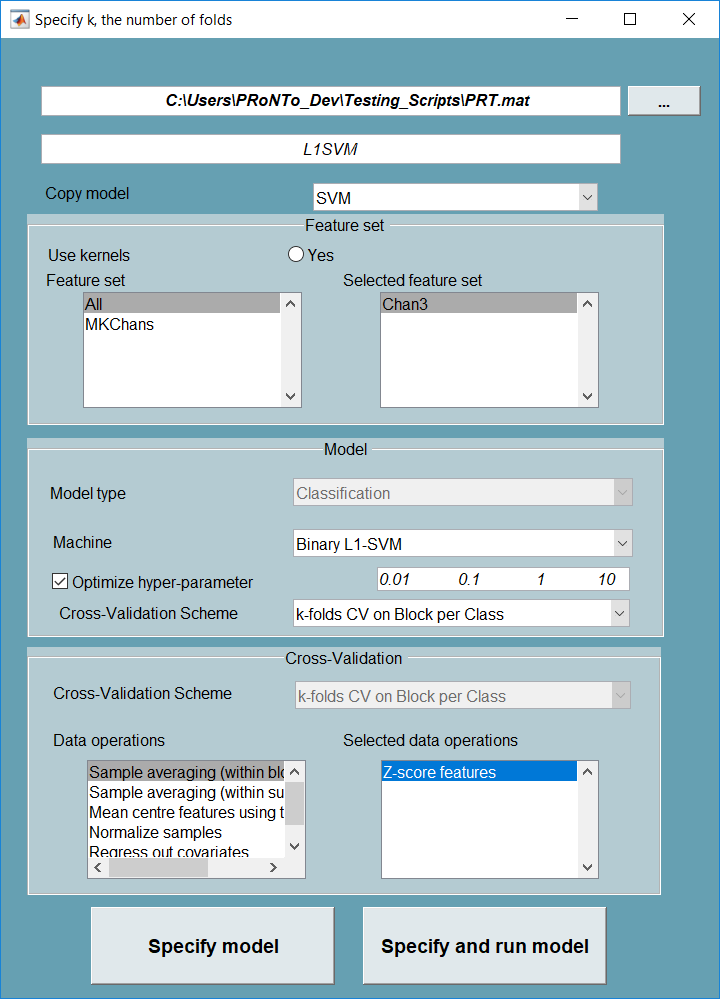
\includegraphics[scale=0.55]{images/Tutorial/v3/non_kernel_machine_tutorial/non_kernel_gui_specify_model_from_final.png}
	\caption{`Model: Specify from' GUI for the new `L1SVM' model.}
	\label{fig:non_kernel_gui_specify_model_from_final}
\end{figure}

%---------------------------------------------------------------------

\subsection{Model: Run}

\begin{itemize}

\item  It is now time to run our models so open the `Run' module.

\item After you select the `PRT.mat' file you will see the 2 models we have created so far. You can either select and run them one by one, or you can select all and run them all together.

\item In `Permutations' select `Perform permutation test', with 100 repetitions. Be aware that 100 repetitions is a small number when running permutation tests and we are only using it for demonstration purposes. 1000 repetitions (or even more) is a more realistic number if you want your results to have a good statistical power.

\end{itemize}

The `Run' window should look similar to the one in figure \ref{fig:multimodal_face_gui_run_final} of Chapter \ref{sec:multimodal_face} with the `Save permutation parameters' option unchecked.



%---------------------------------------------------------------------

\subsection{Display results}

The `L1SVM' model gives 67.21\% total accuracy and a AUC of 0.76, which is worse than the kernel `SVM' model that had a 93.86\% total accuracy and a AUC of 0.99. The results for the `L1SVM' model are shown in figure \ref{fig:non_kernel_gui_display_results}.

\begin{figure}[!h]
  \centering
		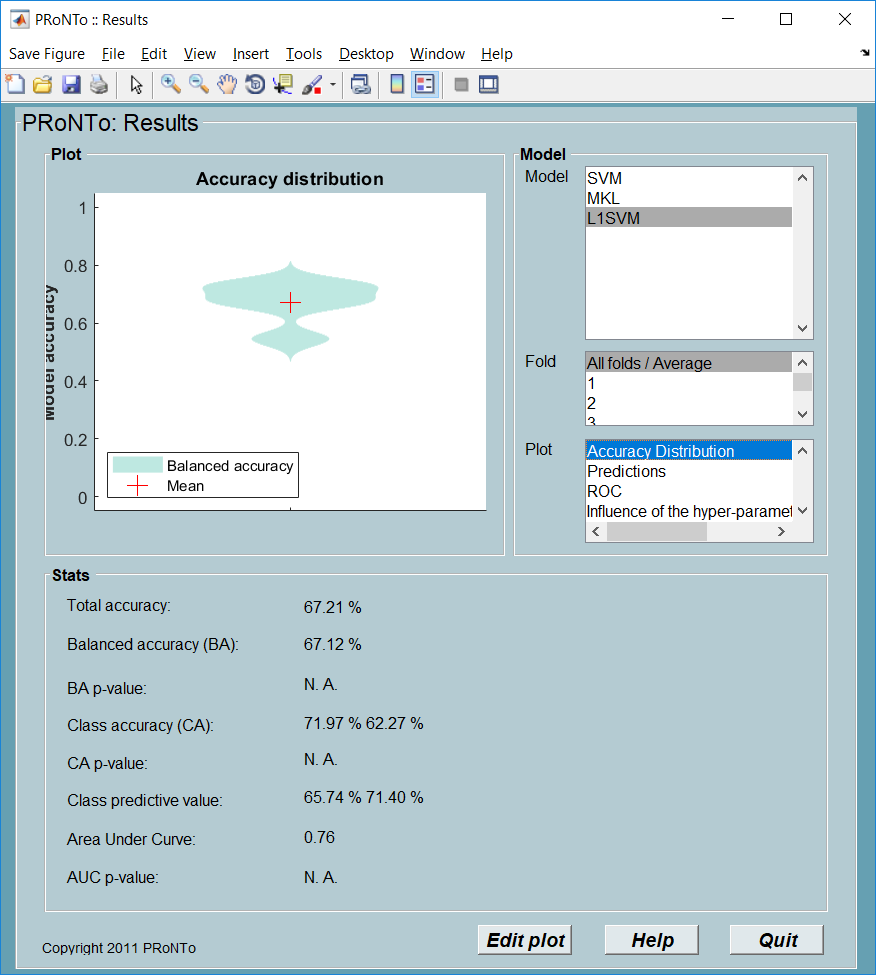
\includegraphics[scale=0.55]{images/Tutorial/v3/non_kernel_machine_tutorial/non_kernel_gui_display_results.png}
	\caption{`Display results' GUI for the new `L1SVM' model.}
	\label{fig:non_kernel_gui_display_results}
\end{figure}
	
%---------------------------------------------------------------------

\subsection{Compute weights}

We can now build the weights for the `L1SVM' model. In this case, select the PRT.mat, the `L1SVM' model and leave the other options as default.

%---------------------------------------------------------------------

\subsection{Display weights}

The weights for the `L1SVM' model are displayed in figure \ref{fig:non_kernel_gui_display_weights}. As this is an L1-SVM, only a few time points on channel 3 should have non-null weights. Even though the L1SVM provides sparse weights for each fold, the average weight across folds, shown in figure \ref{fig:non_kernel_gui_display_weights}, is not sparse. This reflects the fact that different features are being selected across folds therefore the selection of features across fold is very unstable.

\begin{figure}[!h]
  \centering
		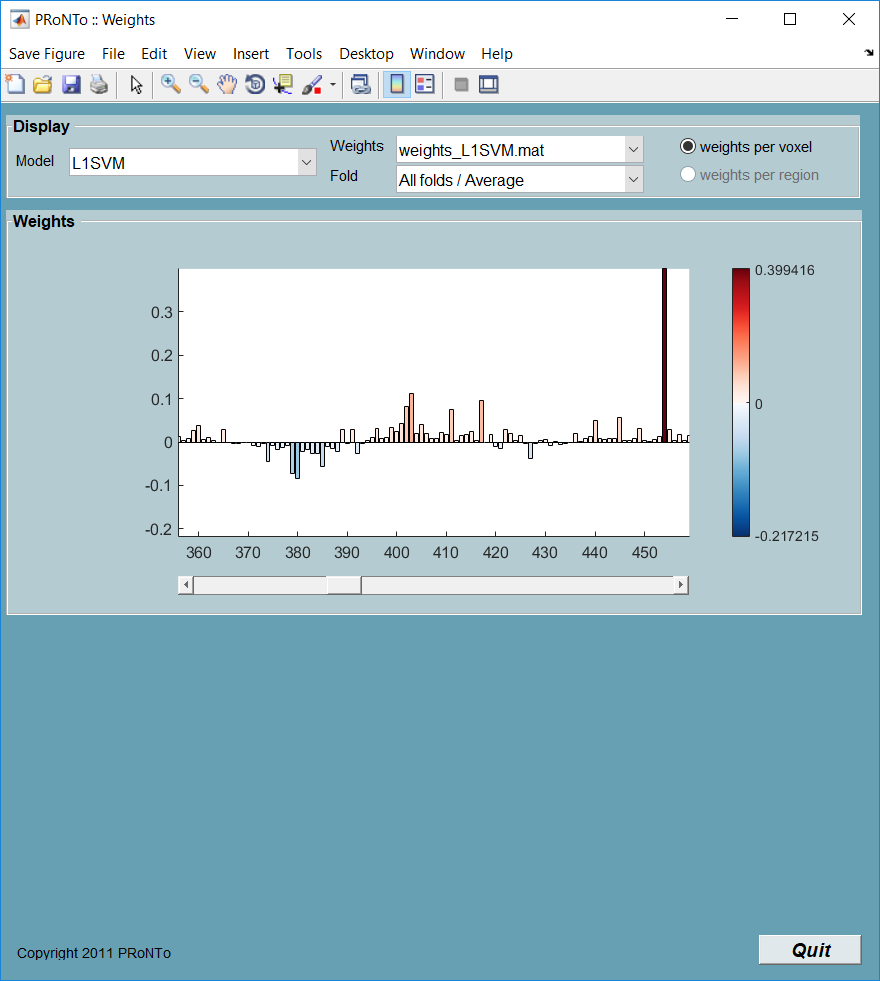
\includegraphics[scale=0.55]{images/Tutorial/v3/non_kernel_machine_tutorial/non_kernel_gui_display_weights.png}
	\caption{`Display weights' GUI. `L1SVM' model.}
	\label{fig:non_kernel_gui_display_weights}
\end{figure}

%=====================================================================



%=====================================================================

\section{Batch analysis}

%---------------------------------------------------------------------

\subsection{Data \& Design}

You will need to replicate, exactly, the procedure followed in the previous chapter. Follow step by step subsection \ref{sssec:data_and_design_semisim_batch} in order to finish inputting the data.

%---------------------------------------------------------------------

\subsection{Feature set / Kernel}

\begin{itemize}

\item First replicate, exactly, the procedure followed in the previous chapter in order to build the first of the two feature sets, `All', used in that chapter. Follow step by step subsection \ref{sssec:feature_set_semisim_batch} in order to do this.

    \item Then build a second feature set (`Chan3'), that will include only channel 3 and time points the same as before, [-100 1100]ms around onset. The final configuration of this feature set should look like figure \ref{fig:non_kernel_batch_prepare_featureSet_3}

\end{itemize}

\begin{figure}[!h]
  \centering
		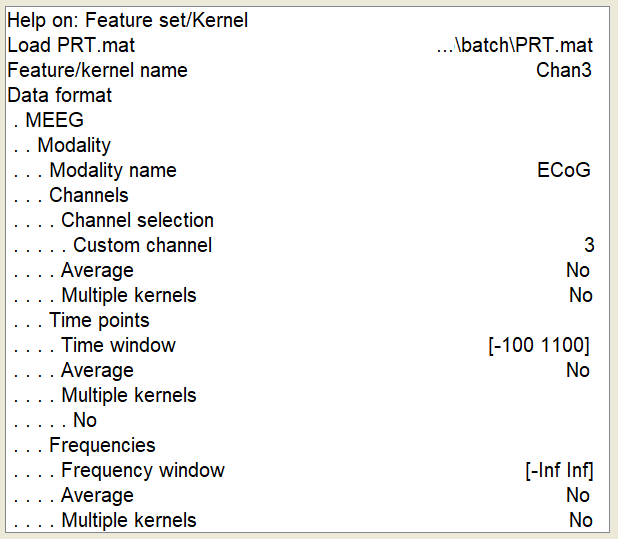
\includegraphics[scale=0.55]{images/Tutorial/v3/non_kernel_machine_tutorial/non_kernel_batch_prepare_featureSet_3.png}
	\caption{`Feature set / Kernel' module in {\tt matlabbatch} for the `Chan3' feature set.}
	\label{fig:non_kernel_batch_prepare_featureSet_3}
\end{figure}

%---------------------------------------------------------------------

\subsection{Model: Specify new}

Replicate, exactly, the procedure followed in the previous chapter in order to build the first of the two models, `SVM', used in that chapter. Follow step by step subsection \ref{sssec:specify_model_new_semisim_gui} in order to do this.


%---------------------------------------------------------------------

\subsection{Model: Specify from}

We will try the `Model: Specify from' {\tt matlabbatch} module and the Binary L2-SVM machine this time. Remember that in the `Model: Specify from' {\tt matlabbatch} module you only need to specify the fields you're modifying from the copied model, and all the rest will remain the same.

\begin{itemize}

\item Specify the appropriate `PRT.mat'.

\item Give a name to the new model (`L2SVM') and choose the model to copy from (`SVM').

\item In the `Fields to modify' select the `New: Field' option.

\begin{itemize}
\item In the `Field', select the `Model type' option, then choose `Classification', `Non-kernel machine' and select the `Binary L2-SVM'.

\item In the `Machine optimization and parameters', select `Optimize hyper-parameter' and choose `k-folds CV on block per class' with a k=4 in the `Cross-validation type for hyper-parameter optimization' field.
\end{itemize}

\item In the `Fields to modify' select once more the `New: Field' option.

\begin{itemize}
\item In the `Field', select the `Feature sets' option, select a `New: Name' and specify it (`Chan3').
\end{itemize}

\item In the `Fields to modify' select once more the `New: Field' option.

\begin{itemize}
\item In the `Field', select the `Data operations' option. Then in `Other operations' select `Select operations', select the `New: Operation' and choose the `Z-score features (Non-kernel only)' option.
\end{itemize}

\end{itemize}

After you have specified everything, the final configuration should look like the one in figure \ref{fig:non_kernel_batch_specify_model_from}.

\begin{figure}[!h]
  \centering
		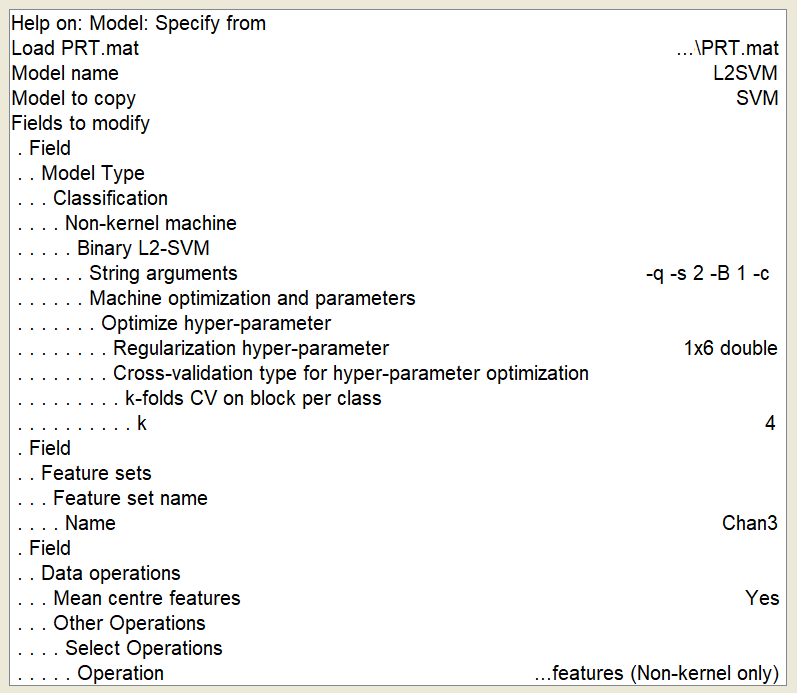
\includegraphics[scale=0.55]{images/Tutorial/v3/non_kernel_machine_tutorial/non_kernel_batch_specify_model_from.png}
	\caption{`Model: Specify from' module in {\tt matlabbatch}.}
	\label{fig:non_kernel_batch_specify_model_from}
\end{figure}


%---------------------------------------------------------------------

\subsection{Model: Run \& Display results}

Simply load your `PRT.mat' and run all the models with no permutations. The model displays an accuracy very similar to the `L1SVM' model.

%---------------------------------------------------------------------

\subsection{Compute \& Display weights}

Open the `Compute weights' {\tt matlabbatch} module, load the PRT.mat, specify the model name (`L2SVM') and leave all the rest at their default values.
\\

In figure \ref{fig:non_kernel_batch_display_weights} you see that the weights for this model are quite smooth compared to the L1-norm. That was expected since the L2-norm produces non-sparse weights.
\\

\begin{figure}[!h]
  \centering
		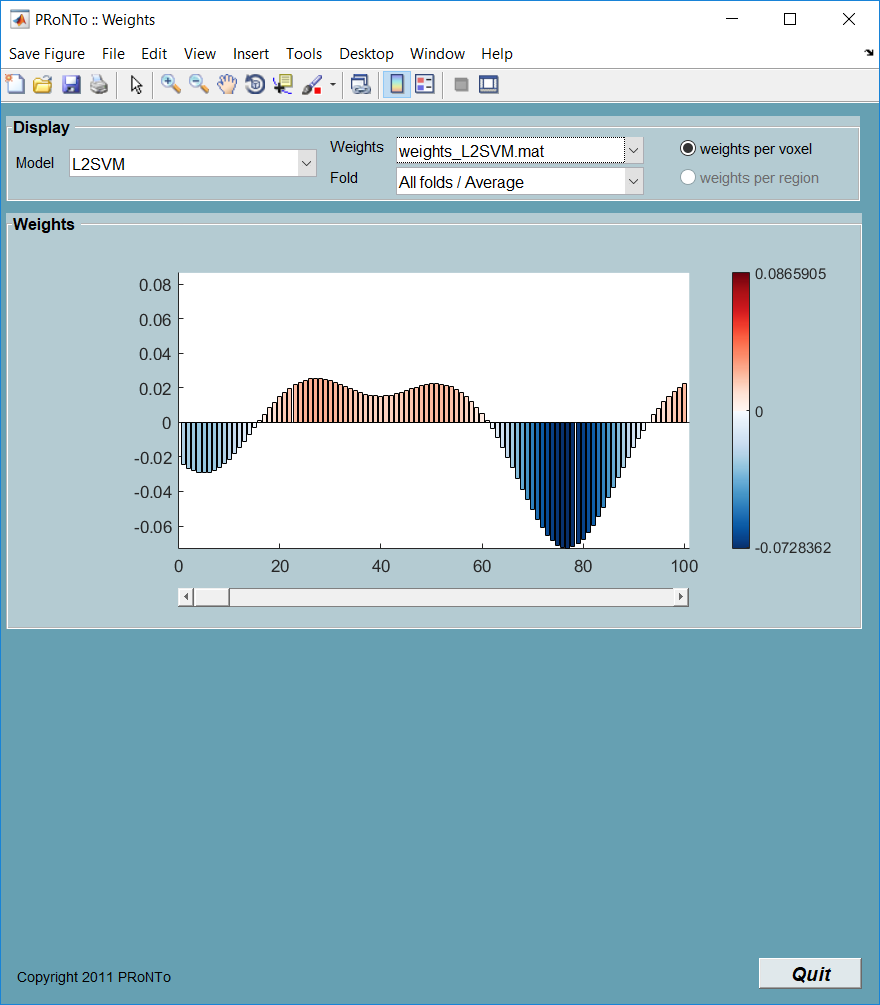
\includegraphics[scale=0.55]{images/Tutorial/v3/non_kernel_machine_tutorial/non_kernel_batch_display_weights.png}
	\caption{`Display weights' GUI for the `L2SVM' model.}
	\label{fig:non_kernel_batch_display_weights}
\end{figure}







